\documentclass[12pt]{amsart}
\usepackage{amsaddr}
\usepackage{marktext} 
%% Remove draft for real article, put twocolumn for two columns
\usepackage{svmacro}
\usepackage[utf8]{inputenc}
\usepackage{lineno}
\usepackage[style=alphabetic, backend=biber]{biblatex}
\addbibresource{bibliography.bib}

%% commentary bubble
\newcommand{\SV}[2][]{\sidenote[colback=green!10]{\textbf{SV\xspace #1:} #2}}

%% Title 
\title{ MATH 102: Ideas  of Math }
\author{ Worksheet 8 }

\date{Nov 6, 2023}

\begin{document}

\maketitle

\section{Concepts}

\begin{definition}
    We call a relation from $A$ to $A$ a relation on $A$.
\end{definition}

\begin{definition}
    Let $R$ be a relation from $A$ to $B$ and $S$ be a relation from $B$ to $C$.
    We define the \emph{composition} of relations $S\circ R$ as follows
    \begin{equation*}
        S \circ R = \set{ (a,c) \in A\times C \st \exists b \in B, (a,b) \in R \wedge (b,c) \in S  }\,.
    \end{equation*}
\end{definition}

\begin{definition}
    Suppose $R$ is a relation from $A$ to $B$.
    The \emph{inverse} of $R$ is the relation $R^{-1}$ from $B$ to $A$, defined as follows:
    \begin{equation*}
        R^{-1} = \set{(b,a)\in B\times A \st (a,b) \in R}
    \end{equation*}
\end{definition}

\begin{definition}
    Suppose $R$ is a relation on $A$.
\begin{enumerate}
    \item $R$ is said to be reflexive on $A$ (or just reflexive, if $A$ is clear from context) if $\forall x \in A (xRx)$, or in other words, $\forall x \in A ((x, x) \in R)$.
    \item $R$ is symmetric if $\forall x \in A \forall y \in A (xRy \rightarrow yRx)$.
    \item $R$ is transitive if $\forall x \in A \forall y \in A \forall z \in A ((xRy \land yRz) \rightarrow xRz)$.
\end{enumerate}
\end{definition}

\section{Problems}
\begin{problem}
    Let $A = \set{1,2}$.
    \begin{enumerate}
        \item Write down a relation $R$ that describe the following thing from subsets of $A$: $X R Y$ if $X\subseteq Y$. 
        \item Represent this relation in the form of arrows and dots.
    \end{enumerate}
    
\end{problem}


\begin{problem}
    Suppose that $A = \{1,2,3\}$, $B = \{4,5\}$, $C = \{6,7,8\}$, $R = \{(1,7), (3,6), (3,7)\}$, and $S = \{(4,7), (4,8), (5,6)\}$. Note that $R$ is a relation from $A$ to $C$, and $S$ is a relation from $B$ to $C$. Find the following relations:

    \begin{enumerate}
        \item  $S^{-1} \circ R$.
        \item $R^{-1} \circ S$.
    \end{enumerate}

\end{problem}

\begin{problem}
    Suppose $R$ is a relation from $A$ to $B$, $S$ is a relation from $B$ to $C$, and $T$ a relation from $C$ to $D$.
    Prove the following
    \begin{enumerate}
        \item $(R^{-1})^{-1} = R$
        \item $\Dom(R^{-1}) = \Ran(R)$
        \item $\Ran(R^{-1}) = \Dom(R)$
        \item $T\circ (S\circ R) = (T\circ S) \circ R$
        \item $(S\circ R)^{-1} = R^{-1}\circ S^{-1}$
    \end{enumerate}
\end{problem}

\begin{problem}
    Determine whether each relation represented by the graph is reflexive, symmetric, or transitive.
    \begin{figure}[ht]
        \begin{center}
            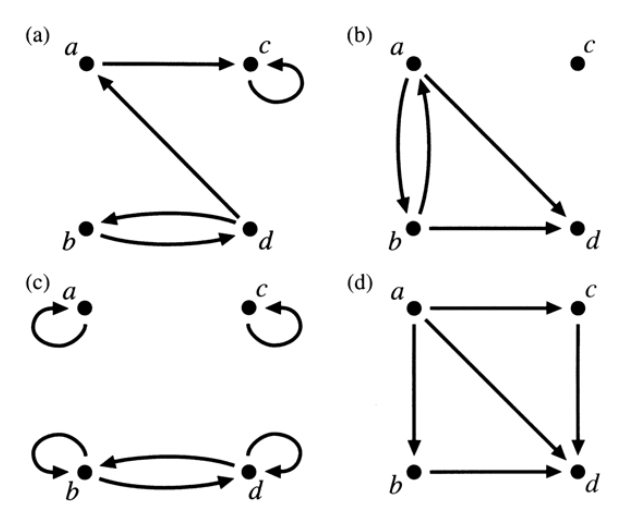
\includegraphics[width=0.95\textwidth]{graph}
        \end{center}
    \end{figure}
    
\end{problem}

\begin{problem}
    Suppose $R$ is a relation on a set $A$.
    Prove
\begin{enumerate}
    \item $R$ is reflexive if and only if $i_A \subseteq R$, where $i_A$ is the identity relation on $A$.
    \item $R$ is symmetric if and only if $R = R^{-1}$.
    \item $R$ is transitive if and only if $R \circ R \subseteq R$.
\end{enumerate}
\end{problem}

\end{document}
